\newpage
\section{Diskussion}
\label{sec:Diskussion}

Das vermessene Magnetfeld ist in Anbetracht der Dicke der Proben relativ
homogen.
Die theoretische effektive Masse von GaAs in Abhängigkeit von der Dotierungsdichte
$N$ in \si{\raiseto{-3}\centi\meter} lässt sich unter Verwendung der
Formel
\begin{equation*}
  \frac{m^*}{m_\text{e}} =
  \num{0.0635} + \num{2.06e-22} \cdot N + \num{1.16e-40} \cdot N^2
  \label{eqn:Theoriewert}
\end{equation*}
berechnen \cite[7]{Nakwaski}. Dabei beziehen sich die errechneten Werte auf eine
Probe bei Raumtemperatur.
Für die beiden verwendeten Proben ergeben sich Theoriewerte von
\begin{align*}
  \frac{m^*_1}{m_\text{e}} &\approx \num{0.065} \\
  \frac{m^*_2}{m_\text{e}} &\approx \num{0.064}.
\end{align*}

Es zeigen sich große Abweichungen zu den experimentell ermittelten
Werten um das fünf- bis achtfache nach unten.
Dies lässt sich auf verschiedene Ursachen zurück führen:
Zum einen war die regelbare Zeitkonstante des einen Photowiderstands
defekt, sodass entstehende Phasendifferenzen zwischen den
Wechselstromsignalen der beiden Widerstände nicht korrigiert werden konnten.
Des Weiteren ließ sich das Signal am Oszilloskop bei der Kalibrierung ohne
magnetisches Feld zwar auf Null herunter regeln, jedoch war dies mit
Einschalten des Elektromagneten nicht mehr möglich.
Aufgrund dieses Rauschens war eine präzise Einstellung mit dem Goniometer
unterschiedlich gut möglich. Bei manchen Frequenz-Probenkombinationen
konnte teilweise über \SI{2}{\degree} keine Veränderung des Signals
erkannt werden. Daher lassen sich die Steigungen der Regressionen
und infolge dessen auch die effektive Masse nur sehr ungenau bestimmen.

Das Rauschen des Signals lässt sich teilweise mit Wärmestrahlung erklären,
welche der Magnet und die Proben aufgrund eines Aufheizens im Laufe
der Messung emittieren. Aus Abbildung \ref{fig:waermestrahlung}
wird ersichtlich, dass die Wärmestrahlung lediglich für die
Wellenlänge von \SI{1}{\micro\meter} nicht beiträgt.
Hier zeigt sich in Abbildung \ref{fig:differenzen} auch
eine signifikant größere Winkeldifferenz.
Schließlich ist zu erwähnen, dass die Filter verstaubt waren und sich
auf den Proben Fingerabdrücke befanden, was zu weiteren Störungen geführt
haben kann.

\begin{figure}
  \centering
  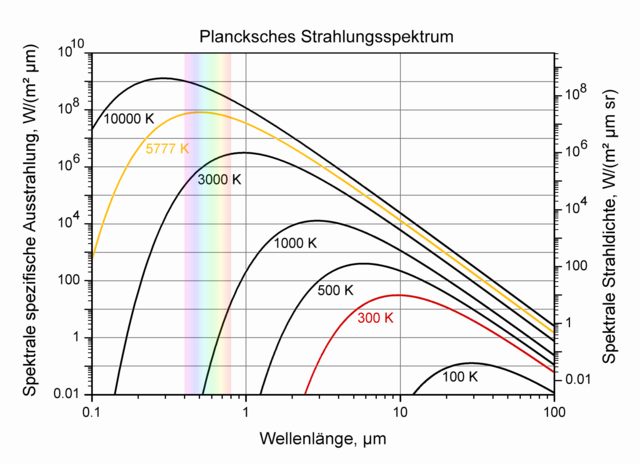
\includegraphics[height=8cm]{images/BlackbodySpectrum.png}
  \caption{Das Plancksche Strahlungspektrum für verschiedene Temperaturen
  und Wellenlängen \cite{waermestrahlung}.}
  \label{fig:waermestrahlung}
\end{figure}
